% This document provides the style to be used for a MSc Thesis at the
% Parallel and Distributed Systems group
\documentclass[11pt,twoside,a4paper,openright]{report}

% use babel for proper hyphenation
\usepackage[british]{babel}
% Graphics: like the DUT logo on the front cover
\usepackage[dvips]{graphicx}
%Enables [H] for figures.
\usepackage{float}
% FONT: times
\usepackage{times}
% for url's use "\url{http://www.google.com/}"
\usepackage{url}

\begin{document}

%%%%%%%%%%%%%%%%%%%%%%%%%%%%%%%%%%%%%%%%%%%%%%%%%%%%%%%%%%%%%%%%%%%%%%%%%%%%%%%
\hoffset=1.63cm
\oddsidemargin=0in
\evensidemargin=0in
\textwidth=5in

%%%%%%%%%%%%%%%%%%%%%%%%%%%%%%%%%%%%%%%%%%%%%%%%%%%%%%%%%%%%%%%%%%%%%%%%%%%%%%%
\parindent=1em

\pagestyle{empty}

% FRONTCOVER
\begin{titlepage}

\null\vfill

\begin{center}
\LARGE{MultiChain:\\
       		an incremental step in a new distributed data structure}
\end{center}

\vspace{1.5cm}

\begin{center}
Steffan D. Norberhuis\\
steffan@norberhuis.nl
\end{center}

\vfill

\begin{figure}[!b]
\centering

\includegraphics[width={0.5\textwidth}]{pics/TUD_logo_color.eps}
\end{figure}

\vspace{2.0cm}

\end{titlepage}


% EMPTY PAGE
\cleardoublepage

\pagestyle{plain}

% TITLE PAGE: page i (hidden)
\begin{titlepage}

  \begin{center}
  \null\vfill
    \begin{center}
    \LARGE{MultiChain:\\
		an incremental step in a new distributed data structure}
    \end{center}

    \vspace{3cm}

    \begin{large}
    Master's Thesis in Computer Science
    \end{large}

    \vspace{1.5cm}

    \begin{normalsize}
    Parallel and Distributed Systems group\\
    Faculty of Electrical Engineering, Mathematics, and Computer Science\\
    Delft University of Technology
    \end{normalsize}

    \vspace{2.0cm}

    \begin{normalsize}
    Steffan D. Norberhuis
    \end{normalsize}

    \vspace{1.0cm}

    % <MM> DD, YYYY
    \today            %TODO: #36 Dit is de datum van uitgifte van final versie aan de afstudeer commissie

  \vfill
  \end{center}

\end{titlepage}



% GRADUATION DATA AND ABSTRACT: pages ii and iii (hidden)
%De aankondiging bevat de spreker, titel, plaats, datum en tijd, samenstelling van de afstudeercommissie en een korte samenvatting (maximaal 25 regels).
\thispagestyle{empty}

\noindent \textbf{Author}\\
\begin{tabular}{l}
Steffan D. Norberhuis\\
\\
\end{tabular}\\
\noindent \textbf{Title}\\
\begin{tabular}{l}
MultiChain: a cybercurrency for cooperation\\
\\
\end{tabular}\\
\noindent \textbf{MSc presentation}\\
\begin{tabular}{l}
% <MM> DD, YYYY (like \today)
December 14, 2015
\\
\end{tabular}

\vspace{1.1cm}

\noindent \textbf{Graduation Committee}\\
\begin{tabular}{ll}
% The order of listing the names: Graduation prof, supervisor(s), others ordered by title + alphabetical
%examples:
%prof. dr. ir. H. J. Sips (chair) & Delft University of Technology \\
%ir. dr. D. H. J. Epema           & Delft University of Technology \\
dr. ir. J. A. Pouwelse          & Delft University of Technology \\
dr. A. Iosup                    & Delft University of Technology \\
dr. ir. Z. Erkin                & Delft University of Technology \\

\end{tabular}

\begin{abstract} %de abstract bevat alleen een korte samenvatting van de inhoud van het onderzoek
Peer-to-peer networks are often large, collaborative networks where peers can join openly.
The essence of a collaborative, distributed system is that every node performs tasks for other nodes.
The peers help often in singular interactions and without direct reciprocity.
This allows malicious peers to abuse and freeride public goods.
The network without countermeasures can fall into a tragedy of the commons
where no one helps another and everyone takes advantage of the generosity of peers.
Only when the reputation of a peer is publicly available at scale and peers trust this reputation
can the network escape the problems of free riding and attain high utility for all participants.

This thesis focuses on designing and implementing the first step of a tamper proof reputation system within Tribler.
Tribler is a peer-to-peer BitTorrent system developed at the Delft University of Technology.
This first step, made by this thesis, is to create MultiChain, a proof-of-concept bookkeeping system.
MultiChain tracks the upload and download amounts of peers to eliminate free riding.
MultiChain is cryptographically protected and validated.
The bookkeeping system has to be scalable to be publicly available and be able to process enough transactions.
The system has to work in an asynchronous network.

A new design of a distributed data structure that can be used as a ledger is introduced by this thesis.
This first step with MultiChain is already more resilient to tampering than previous work, like BarterCast.
BarterCast had no security measures against tampering records.
Peers are participants of a peer-to-peer network.
The design of MultiChain is to have a chain of blocks for every peer as a ledger.
A block contains a transaction between a peer.
This block is shared and added to both chains.
This makes both chains of the peers intertwined and entangled at a shared block.
The proposed design abandons the typical global, full ledger.
The protocol of creating these blocks between peers is described.
The problems faced by MultiChain in an asynchronous network are explained.
The thesis proposes how the design can overcome these problems
by only allowing atomic operations to be performed on the chain
and to introduce unfinished blocks in the chain.

The implementation of the design is tested and experimented with within this thesis to validate it to work correctly.
Furthermore, a number of weak points are discussed.
These weak points have to be addressed in the future to create a tamper proof reputation system.



\end{abstract}

\clearpage



\pagenumbering{roman}
\setcounter{page}{4}

% EMPTY PAGE: page iv
\cleardoublepage

% OPTIONAL QUOTATION: page v
%\pagestyle{empty}

\null\vfill

\begin{center}
\emph{``TODO QUOTE''} -- TODO QUOTED PERSON
\end{center}

\vspace{10cm}

\clearpage


% EMPTY PAGE: page vi
%\cleardoublepage

% PREFACE: page v
\chapter*{Preface}
\addcontentsline{toc}{chapter}{Preface}
The huge increase in Bitcoin adoption, 
due to the increase in uncertainty in the security of traditional currency 
after the financial crisis in 2008, 
is only rivaled by the speculation of the enormous possibilities 
of the underlying technology of the block chain.
The block chain is the first technology, seen with real world adoption,
that allows to register transactions without a trusted third party.
But the block chain has several limitations in scalabillity 
that will limit Bitcoins in fully replacing traditional currencies with a digital currency.
It also limits block chain as a scalable basis for a large scale reputation system, 
similar to a digital currency, with vast amounts of transactions.
These developments provides motivation to research the properties and possibilities of a variant of the block chain:
MultiChain.

\vspace{1\baselineskip}

\noindent
I would like to acknowledge several people that helped me during my master thesis.
First I would to heartily thank dr.ir. Johan Pouwelse for his mentoring and helping me in setting goals and achieving these goals.
Furthermore I would like to thank dr.ir. Cor-Paul Bezemer for his guidance and help with implementing within Tribler. 
I also would like to thank Elric Milon and Lipu Fei for answering countless questions
and problems I encountered during the programming phase of my thesis.
For the excellent feedback and help to improve my code I would like to thank dr.ir. Niels Zeilemaker.
His support by adding functionality to Dispersy was also invaluable.
Rob Ruigrok was doing his master thesis at the same time
and helped me to avoid problems he encountered before I experienced them as well and
I am grateful for this help.
I am also very thankful for the companionship I felt within my work room 
and I would like to thank especially Hans Bogerts BSc, Niels Doekeijmeier BSc and Ernst van der Hoeven BSc.
You certainly made my work more enjoyable.

\vspace{1\baselineskip}

\noindent
Steffan Derk Norberhuis

\vspace{1\baselineskip}

\noindent
Delft, The Netherlands

\noindent
\today

% EMPTY PAGE: page vi
\cleardoublepage

% TABLE OF CONTENTS: starting at page vii
\tableofcontents

\cleardoublepage

\pagenumbering{arabic}
\setcounter{page}{1}




% CHAPTERS ... For instance: History/Prior Work, Design/Implementation, Experiments
% INTRODUCTION
\chapter{Introduction}
\label{chp:introduction}
Tribler is a peer-to-peer file sharing program developed by the Delft University of Technology for research purposes.
Tribler expands the BitTorrent protocol and has added multiple improvements on this protocol.
The main focus of Tribler is to make security and privacy the default for Internet users and impossible to shutdown.
A fully distributed program, not relying on any central component, is needed to achieve this.
Tribler has been designed and build using this methodology\cite{Pouwelse-tribler}\cite{Bakker-tribler}.
This master thesis was conducted as part of the research mission to improve Tribler.

\vspace{1\baselineskip}

\noindent
TODO ORGANISATIONAL DESCRIPTION OF THESIS

\section{Tribler}
%TODO update
In peer-to-peer file sharing a node called a seeder uploads parts
of a file to another node, the downloader.
The role of being a seeder and downloader constantly changes
and a node can be both at the same time for different, parallel connections.
A seeder can become a downloader when they wish to download other files
and downloaders can become seeders,
if they posses a file someone else wants.
The ratio between the total size downloaded and uploaded is called the seeding ratio\cite{Cohen-bittorrent}.
private community source

The uploading can be seen as an interaction of one node helping another node.
These interactions comes at the cost of consuming bandwidth for both parties.
There is only direct benefit for the downloader.
The downloader receives a file he wants.
There is no direct barter between the seeder and downloader.
As the seeder does not get anything in return for uploading the file.
Although it can happen by chance that a downloader is also a seeder directly to the original seeder,
but this is unlikely\cite{Lai-Incentives}.

If everyone contributes, files become more available and are downloaded at higher speed.
This claim is supported by measurements taken in private communities
\cite{meulpolder-privatecommunities}.
In private communities high seeding ratio's are enforced by a third party.
Both high availability and high download speeds result in a higher utility for the downloaders.
But currently freeriding in these networks takes places in high quantities\cite{Adar-Freeriding},
The BitTorrent Tit-for-Tat protocol is not enough to stop abuse\cite{Pouwelse-tribler}.

Tribler wants to achieve a high global seeding ratio by making it benificial to have such a ratio.
Nodes can award each other with higher cooperation if a node has a reputation itself to be cooperative.
This requires for a tamper-proof interaction history to base a reputation on in a network.
Those contributing more receive more help in return,
and malicious nodes cannot abuse the network by tampering with the interaction history.

Tribler has recently implemented anonymous connections using onion routing.
This feature allows downloaders to become indistinguishable from other users in the network.
But every data packets has to be forwarded
by a number of intermediate hop between the downloader and seeder\cite{Plak-anonymous}.
The requirement of forwarding packets increases the network load of data being sent.
The total cost of bandwidth per file is increased,
but also the number of nodes helping a single node downloading a file increases.
This in turn increases the necessity of an incentive system to reward collaboration.


%Problem description
\chapter{Problem Description}
In a distributed system nodes will have interactions with other peer nodes.
A node will have to decide how to react to these peers.
Our work is beneficial to the process of deciding how to react to these peers.

In this chapter the problem will be described of how to decide to react to a peer.
The problem will first be explained in a simplified form.
Using this simplification, the problem will be transformed gradually
to the real world problem faced in distributed systems today.
Finally several real world examples of the problem will be described.

\section{Deciding to help}
Nodes can decide to cooperate with a peer or decide not to help a peer and defect.
This is the traditional Prisoner's Dilemma 
and we will explain this dilemma\cite{Nowak-PrisonerDilemma}\cite{Lai-Incentives}.
Nodes can help each other at a cost, a negative utility, 
but the recipient of the help will receive a beneficial utility from the help.
The benefit received is greater than the cost and is denoted by $R$ for reward.
But if one node chooses to not help the other node,
 then he will still receive a beneficial utility and at no cost, $T$ for temptation.
The node that provided the aid will now receive no benefit and only incur a cost $C$.
If both nodes choose to not help each other, 
then they will both receive a penalty $P$, which is higher then the cost of helping each other.

This dilemma can be repeated several times with the same nodes and is the Iterated Prisoner's Dilemma.
Each time both nodes will have to decide if it will help the other node.
The utility received can be seen in Table \ref{tab:pd-um}.

\begin{table}[h]
\center
	\begin{tabular}{l|ll}
	A\textbackslash B       & cooperate  & defect     \\ \hline
	cooperate & $R_A /R_B$ & $T_A /C_B$ \\
	defect    & $T_A /C_B$ & $P_A /P_B$
	\end{tabular}
\caption{Prisoner's Dilemma utility matrix}
\label{tab:pd-um}
\end{table}

A rational node wants to receive maximum benefit at a minimal cost.
The node will follow a strategy that he believes will achieve this.
At first it might seem that a node will always choose to defect,
because it will never incur a cost and receive maximal benefit.
But the other node will be reluctant to help a node if the aid is never returned.
Simple strategies, like tit-for-tat or win-stay, lose-shift, suffice in the Iterated Prisoner's Dilemma
and will perform well\cite{Nowak-Cooperation}.

In a large scale, distributed system, this dilemma occurs with every interaction between nodes.
The node can already be familiar with the peer,
but more often the peer will be a peer the node has not interacted with before.
A further complication is that help is one way and can no longer be exchanged.
This complication excludes the direct opportunity to barter for help 
or to barter for help in the future\cite{Lai-Incentives}.
The performance of the tit-for-tat or win-stay, lose-shift strategies
quickly deteriorate in such a situation.

For a node it is easier to abuse the generosity of others in this more anonymous situation.
Nodes that help others will be penalized through the cost they incur
and incentivized to adopt the malicious behavior themselves.
Nodes in general will become more reluctant to help nodes\cite{Nowak-PrisonerDilemma}.
In the end no node will help another and all nodes will receive a penalty.
This is commonly called the Tragedy of the Commons in the literature \cite{hardin-tragedy}.
The whole network will actually receive more benefit in total if everyone would corporates.
But nodes have no way of knowing if the peer they meet are willing to help.

\section{History of decisions}

In the Iterated Prisoner's Dilemma the history of the previous transactions can be used 
to see if a node helped others in the past.
The simple strategies, previously mentioned, use a history to improve performance
to avoid getting abused.
But this private history is not effective to achieve high overall utility in distributed systems,
because the peers are often interacted with for the first time.
No history is known for these peers.
A public history of node, containing every previous interaction, is necessary to prevent abuse
and is able to achieve high overall utility\cite{Lai-Incentives}.

A history can be used to create a currency or a reputation system.
The node providing help will receive a boost in currency or a beneficial reputation.
The currency or reputation can be used in the future to receive aid.
In a currency system, receiving help will transfer currency to the helper.
In a reputation system, only nodes with a sufficiently good reputation will be helped.

The currency or reputation has to be made publicly available to all nodes in the network.
But a node publicizing to hold a certain reputation is not sufficient as it is not trustworthy.
So a interaction history, that contains every prior interaction a node has conducted, is publicized.
Nodes can cross-reference the interaction history with other nodes and calculate the amount of currency 
or the reputation that a node has.
Based upon this calculation, the node can decide to provide aid or not.

The interaction history has to be distributed among the nodes in the network
to become publicly available.
Efficient distribution protocols are a difficult challenge themselves and outside the problem scope.
But distribution is worth mentioning, because it puts constraints on the interaction history.
The interaction history has to be distributable in an efficient manner.
Only if it meets these constraints, will an interaction history be usable in a distributed system.

\section{Tamper-proof to facilitate thrust}

Interaction histories only prevent direct abuse of the generosity of the nodes.
A malicious node can still try to tamper with the interaction history.
An example of a type of these attacks are double spending attacks\cite{Nakamoto-bitcoin},
where a interaction is altered.
But a node can also try to deny an interaction.
The interaction history has to be resilient to attacks that tamper the interaction history, 
or no one will trust the history.

A digital currency system builds upon trust just as much as a banknote currency.
A reputation system will also need a level of trust.
A system cannot be fully secure, 
but still a reasonable certainty can be achieved that no tampering of the interaction history can occur.
Reasonable certainty is for example that no attack can happen 
if more than half of the network consists of honest nodes.

\section{Real world examples}
In this section we will describe real world problems of the problem type introduced.
This is meant as an illustration of the real world problems and is not a complete survey.

Ad hoc networks are networks that rely on the willingness of nodes to cooperate
and forward messages to each other.
These messages are forwarded at a cost to the node.
For example, the cost can be the power consumption, 
which is limited due to the node running on battery power.
Energy efficiency becomes a prime concern for these node. 
Every node may not display the same willingness to forward messages and be more selfish.
Protocols that use currency or reputation are already proposed
for this problem\cite{Anderegg-AdHoc}.

In BitTorrent networks nodes help each other to download files by sharing chunks of files.
Especially in these networks are interactions with the same node infrequent\cite{Lai-Incentives}.
Cooperating nodes should receive more aid in the form of higher download speed,
then the nodes that feed upon the network and contribute no upload speed to the network.
It has been shown that in these network
free riding takes place in large quantities\cite{Adar-Freeriding}.

%Related work
\chapter{Related Work}
In this chapter we will discuss related work on tamper-proof interaction histories.

\section{Bitcoin}
Bitcoin is a digital currency that uses a interaction history 
to keep track of transactions made between nodes.
The interaction history is a datastructure called the block chain.

The block chain imposes limits on Bitcoin in several ways.
These limitations on Bitcoin can be seen as the initial motivation for our work.
How Bitcoin uses the block chain technology will be introduced first.
In the following, the limitations imposed by the block chain will be explained.

We will only introduce how Bitcoins uses the block chain and why it does so in such a way.
This section is not a full explanation of the Bitcoin protocol
and only discusses relevant parts of the Bitcoin protocol.
The best starting point for a full explanation of Bitcoins 
is the original paper by Nakamoto\cite{Nakamoto-bitcoin}.
Further information and improvements on Bitcoin can be found on the Bitcoin website\cite{Bitcoin.org-site}.

\subsection{Block Chain}
For a currency to work, people have to be able to trust with a reasonable certainty that no double spending can occur.
Double spending With physical tokens is impossible,
but the same guarantee is not trivial for digital currencies without a trusted third party.
Bitcoin has multiple safe gaurds that work together to prevent double spending.
These safe gaurds will be introduced during the explanation of how Bitcoin works.

The core of the Bitcoin protocol is the block chain.
The block chain contains every transaction of bitcoins.
A transaction consists of three parts.
The first part is the public key the new owner of the bitcoin.
The hash of the whole, previous transaction and the public key of the new owner is concatenated.
This concatenation is hashed and this hash is the second part of the transaction.
The third final part is signature by the current owner of the hash of the concatenation.
The previous transaction is a transaction of the same bitcoin.
The ownership of the bitcoin by the current owner can be verified
by verifying the whole history of the bitcoin.
A transaction is usually shortend to Tx in Bitcoin related work and is used in images in this report.

\begin{figure}[H]
	\centerline{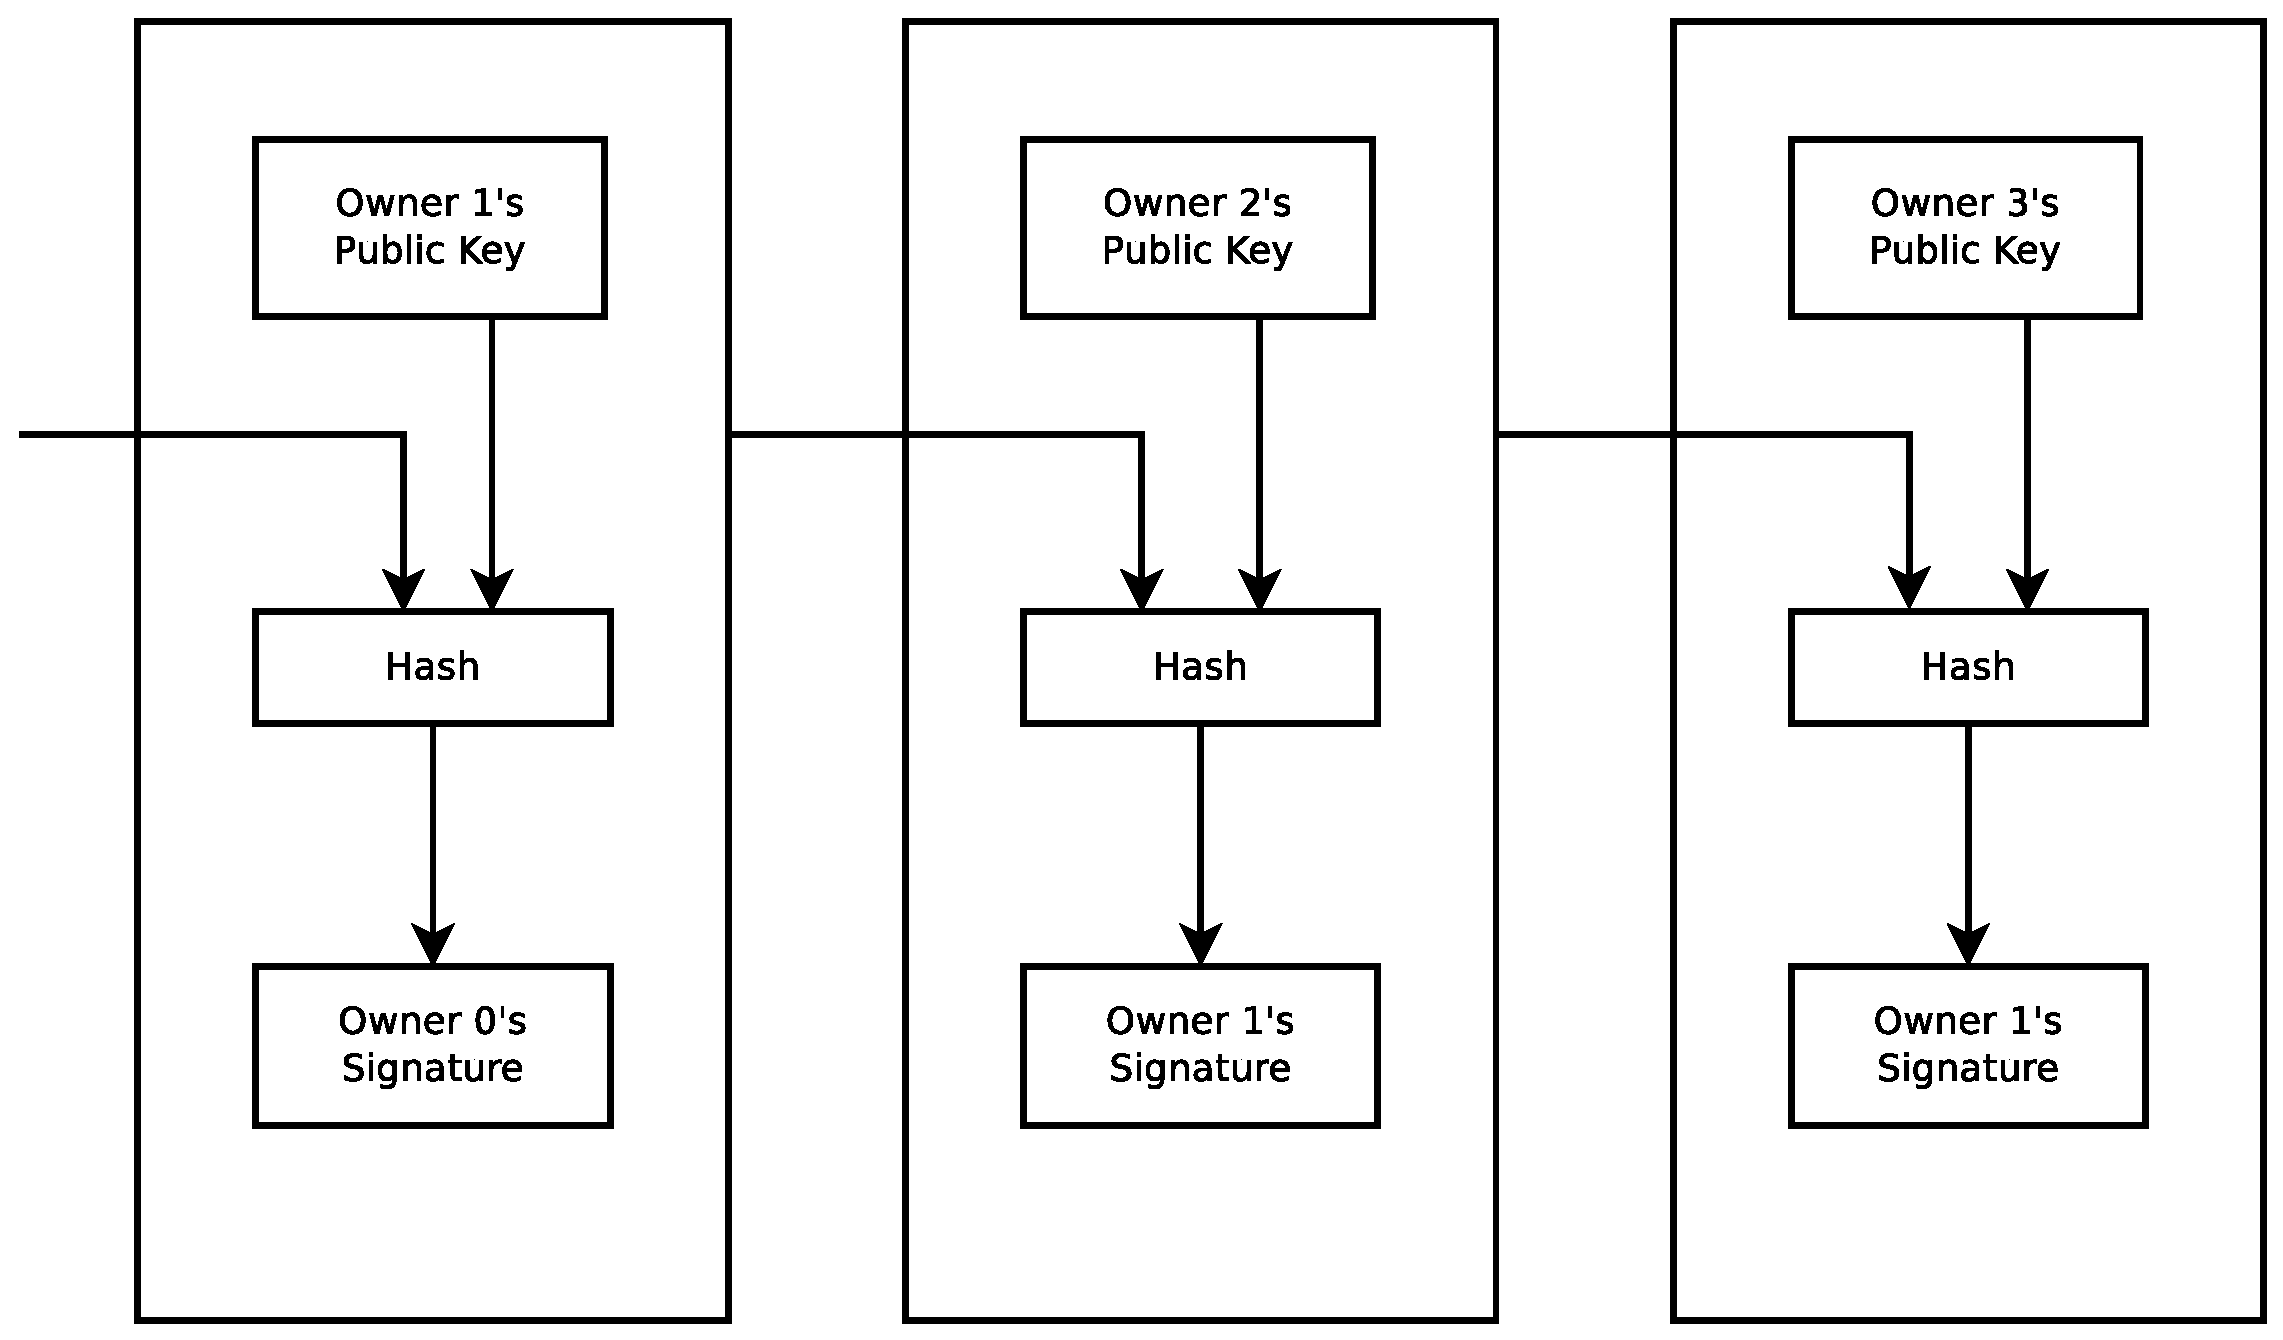
\includegraphics[scale=0.3]{relatedWork/figs/transactions.eps}}
	\caption{Transaction chain}
\end{figure}

Multiple transactions are aggregrated into a single block.
Every block contains the hash of the previous block.
This creates the block chain.
Transaction chains across span several blocks inside the block chain.

These blocks are created by nodes in the network, so called miners.
A miner receives transactions from other nodes in the Bitcoin network.
An attacker can malicously transmit transactions to double spend a bitcoin he owns or does not have.
So every transaction is verified on arrival at a node.
Any transaction that is invalid is just dropped by the node.
No penalty is awarded to the malicous attacker.

The transactions are received in a non deterministic way induced by network characteristics.
The non deterministic nature causes blocks to differ from miner to miner.
The order of transactions has to be agreed upon by the network to eliminate this inconsistency.

Bitcoin uses election to pick the next block  based upon a Proof-Of-Work system.
A nonce is added to every block. 
This nonce is just a number that can be varied,
but is only sound if the hash of the whole block starts with a certain number of zeros.
Miners have to find the correct nonce for their block and this is a proof of work.

\begin{figure}[H]
        \centerline{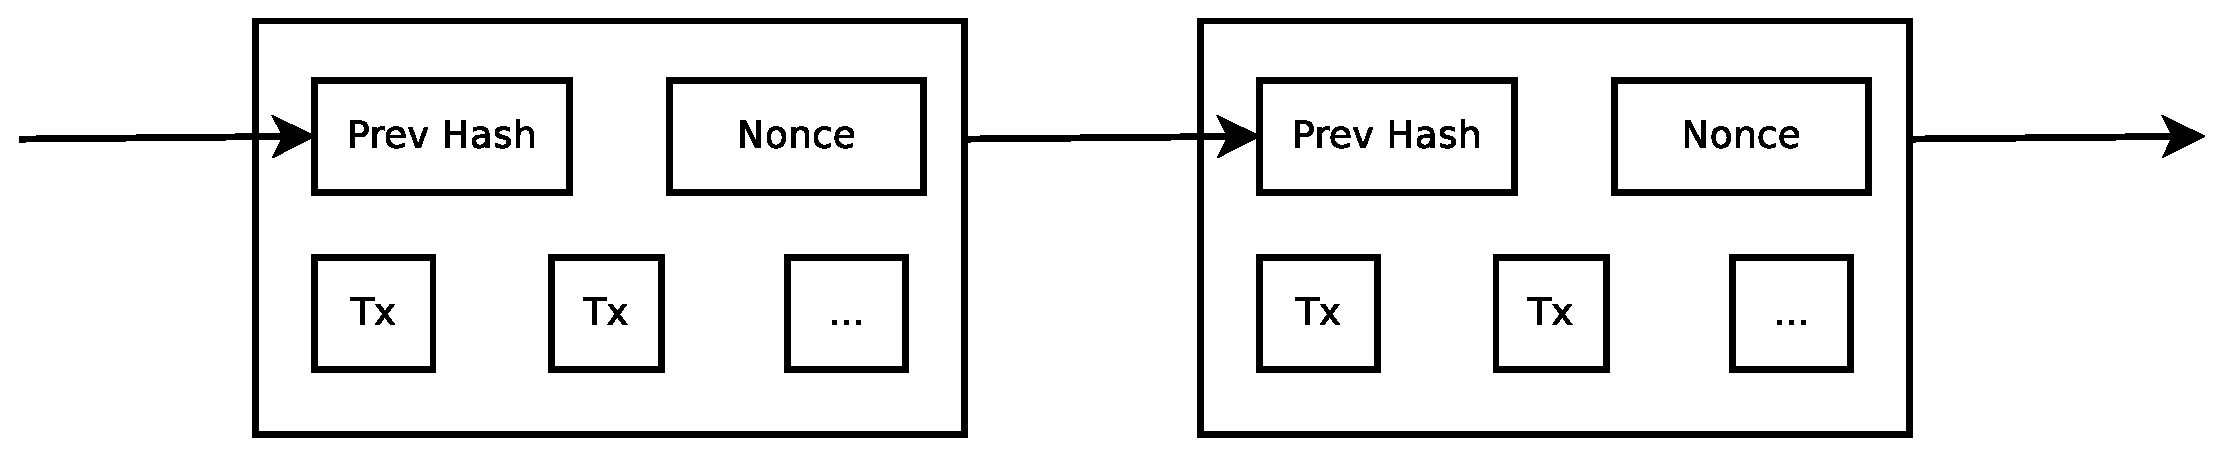
\includegraphics[scale=0.3]{relatedWork/figs/blocks.eps}}
        \caption{Block chain}
\end{figure}

But miners can still find a valid nonce at approximately the same time
and notify parts of the network of their newly found block.
This leaves the network again in an inconsisted state.
These multiple versions of the next block attached to the previous block can be seen as branches.

To solve this inconsistency, Bitcoin nodes save both branches and continue using the longest branch.
At some point one branch will become predominant in the network.
More nodes will dedicate compute power to extend this branch and the growth rate will increase for this branch.
The faster growth rate will ensure that the branch will be adopted by the network as a whole.

The amount of zeros needed in the hash is adjusted to compensate for the fluctuating speed of the network to be able to find nonces.
This is called the hash speed and is the amount of hashes calculated per second.
The hash speed of the Bitcoin network has increased nine fold.
The amount of zeros balances the probability of branches occuring
and the time before a new block is found,
which in turn is how fast transactions are processed.
The growth of the hash speed can be seen in \ref{fig:hash-speed}.

\begin{figure}[H]
        \centerline{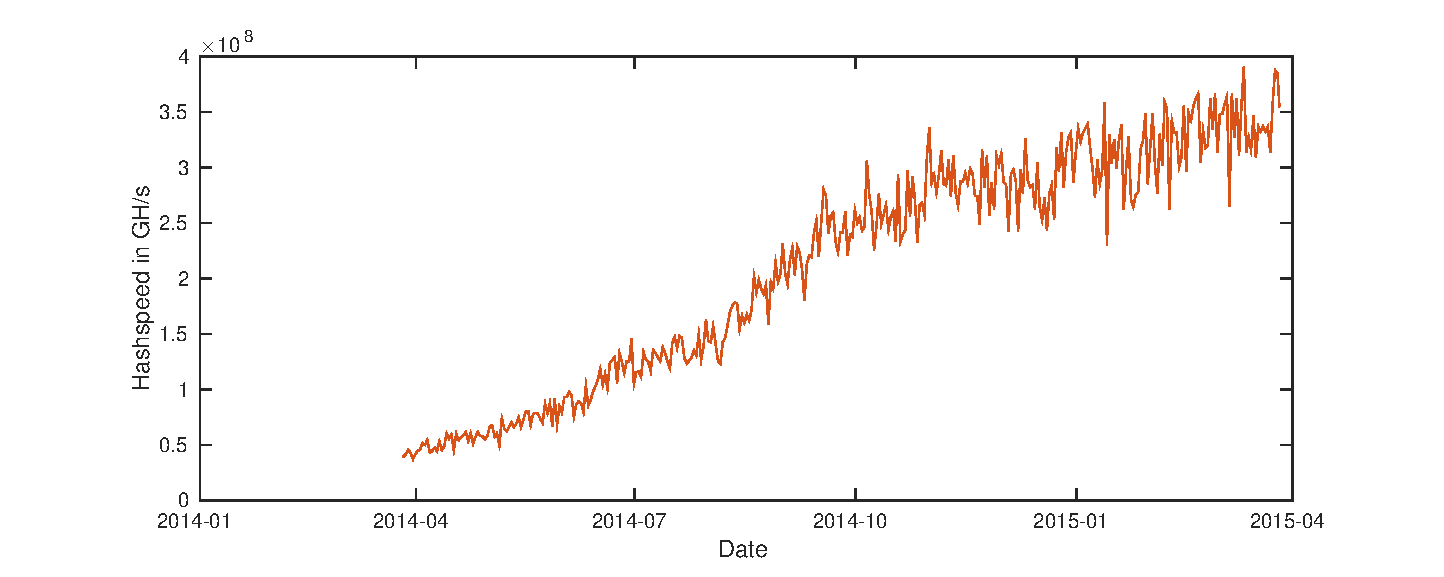
\includegraphics[scale=0.6]{relatedWork/figs/hashspeed/hashspeed.eps}}
        \caption{Amount of hashes calculated per second in the Bitcoin network.\cite{Blockchain.info-bcs}}
	\label{fig:hash-speed}
\end{figure}

Another possible attack to double spend a bitcoin is by sending a transaction to one part of the network,
but to the other part of the network a transaction with a different receipient.
It is possible that both transactions will be introduced into the block chain, but in different branches by two independend miners.
Eventually one branch will win and the attack is averted.

The behaviour just described makes that a transaction can never be confirmed with full certainty.
Another branch could possibly always over take the current longest branch.
This also makes the network vulnerable if the total compute power is owned by a malicous attacker is more than the total compute power of the honest nodes, 
even if the attack has control of 51\% of the compute power. 
In the end the current branch can be overtaken by a new branch started by the attacker.
This new branch allows the whole transaction history to be rewritten by the attacker.
Bitcoin introduces points in the chain that are to be considered final and can no longer change.

\subsection{Limitations}
In this section we will discuss the several limitations of Bitcoins
that originate from the use of the block chain.

\subsubsection{Size}
To be able to prevent double spending and rightfull spending by the right owner, 
the node verifying a transaction needs to be aware of the full history of a bitcoin.
This results in that a node needs the entire block chain to verify a transaction.

The block chain is a data structure ever increasing in size.
No block or data contained in that block is removed.
The block chain has been growing since its inception in 2009.
The size and growth can be seen in figure \ref{fig:bc-size}.

\begin{figure}[H]
        \centerline{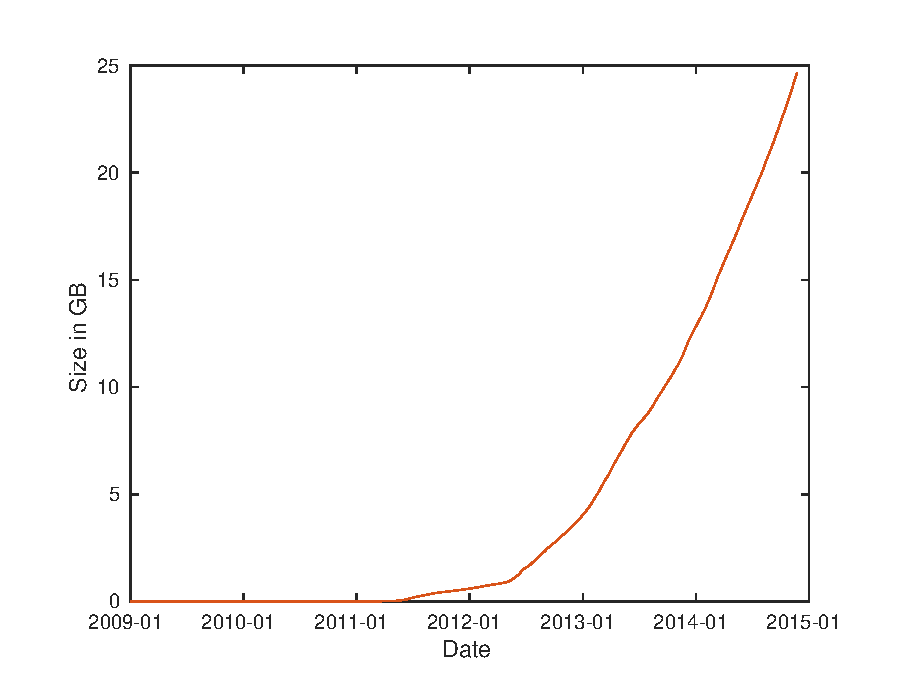
\includegraphics[scale=0.6]{relatedWork/figs/blockchainsize/blockchainsize.eps}}
        \caption{The size of the block chain.\cite{Blockchain.info-bcs}}
	\label{fig:bc-size}
\end{figure}

The size of the block chain at time of writing already prevents less powerfull devices
to operate on the block chain.
This problem is only going to become bigger with the continued creation of transactions
and at a faster pace due to increased adoption of Bitcoin.

This problem was already identified by Nakamoto in his original paper on Bitcoin.
The paper proposes Simplified Payment Verification (SPV).
In SPV mode a node only downloads the block headers of the longest chain.
If a transaction is to be verified, it requests from the network the specific transaction
along with a Merkle tree linking it to a block in the chain.
The Merkle tree can be used to verify that the transaction was included into the block chain.
This allows to calculate with some confidence that the transaction was accepted.

SVP only gives reasonable confidence and is not as secure as running a full node.
Trust has to be placed in the nodes that send the block headers and Merkle Trees.
Secondly, a transaction that is recorded in a more recent block is less difficult to tamper with
than a transaction deep down in the block chain.
This is only an acceptable solution for clients willing to accept more risk due to having a less secure system.
Therefor it is not a solution for the problem for every one.




% BIBLIOGRAPHY
\bibliographystyle{bib/latex8}
\bibliography{bib/bibliography}

%\appendix

%\include{appendix_a}

\end{document}

